\section{Robustness}
The field measurements showed.
\cite{smolnik_5g_2020} \SI{3}{\metre} corn plants
Therefore, the following section focuses on the influence of the different physical layer parameters on the robustness of the IEEE 802.11ax standard
Wi-Fi transmissions.
\todo{Why Matlab? Why not ns-3?}
The MATLAB WLAN Toolbox \footnote{\url{https://de.mathworks.com/products/wlan.html?s_tid=AO_PR_info}} is a add-on to simulate, analyse, and test of wireless LAN communications systems.
The WLAN Toolbox supports a wide range of IEEE 802.11 standards.
Since Release R2019b \footnote{https://de.mathworks.com/help/wlan/release-notes.html}, the WLAN Toolbox supports the Signal Recovery, Packet Extension and Physical Layer abstractions to simulation IEEE 802.11ax networks.

My robustness analysis is based on the WLAN Toolbox example wlan/HESUExample \footnote{https://de.mathworks.com/help/wlan/ug/802-11ax-packet-error-rate-simulation-for-single-user-format.html} to simulate the \ac{PER} of point-to-point IEEE 802.11ax networks for
a specified \ac{SNR} values.

First, I set the IEEE 802.11ax physical layer parameters using the wlanHEConfig object, where I define the following default parameters:
\begin{itemize}
	\item \ac{GI} of \SI{3200}{\nano\second}
	\item \ac{BW} of \SI{20}{\mega\hertz}
	\item 2 spatial streams
	\item 2 transmit antennas
	\item \ac{DCM} disabled
	\item \ac{STBC} disabled
	\item \ac{LDPC} enabled
	\item HE-\ac{MCS} of 0
	\item \ac{CR} of 1/2
	\item Extended range mode disabled
\end{itemize}
\todo[color=yellow]{use table?}
Next, I chose a channel model to simulate the channel. The WLAN Toolbox supports a wide range of channel models, such as wlanTGaxChannel, wlanTGnChannel, wlanTGacChannel, and wlanTGnChannel.
The wlanTGaxChannel model supports six different channel models for IEEE 802.11ax networks, named TGax-A, TGax-B, TGax-C, TGax-D, TGax-E, and TGax-F.

As I want to simulate outdoor scenarios, I chose the TGax-F channel model, which is suitable for outdoor scenarios.
The wlanTGaxChannel model supports configuring the \ac{BW}, the number of transmit and receive antennas, which I set equal to the configuration of the wlanHEConfig object.
\cite{freq_plan} allow outdoor transmission in the frequency range of \SI{5.725}{\giga\hertz} to \SI{5.825}{\giga\hertz}. Therefore, I set the carrier frequency to \SI{5.6}{\giga\hertz}.
Additional parameters are left at their default values as they are not relevant for outdoor scenarios.

The simulation runs the following procedure for each specified \ac{SNR} value.

First, the WLAN Toolbox generates a random packet of the specified length of \SI{1000}{\byte}, which is used to create a
Wlan waveform based on the physical layer parameters specified in the wlanHEConfig object using the wlanWaveformGenerator function.
The generated waveform is then passed through the configured wlanTGaxChannel to simulate the channel. The output of the channel model is the received waveform, where
the channel model adds noise to the transmitted waveform based on the specified \ac{SNR} value.

The received waveform is then passed through the wlanWaveformDecoder function to decode the received waveform.

\subsubsection*{\acf{MCS} and \acf{CR}}
In a first simulation run, I analysed the influence of a chosen set of HE-MCS values on the \ac{PER} in regards to the \ac{SNR}.
The results in \autoref{fig:PER_SNR_MCS} show that the \ac{PER} decreases with higher \ac{SNR} for all HE-MCS values. The
\ac{PER} decreases at lower \ac{SNR} values for lower HE-MCS values.
\begin{figure}[H]%
	\centering
	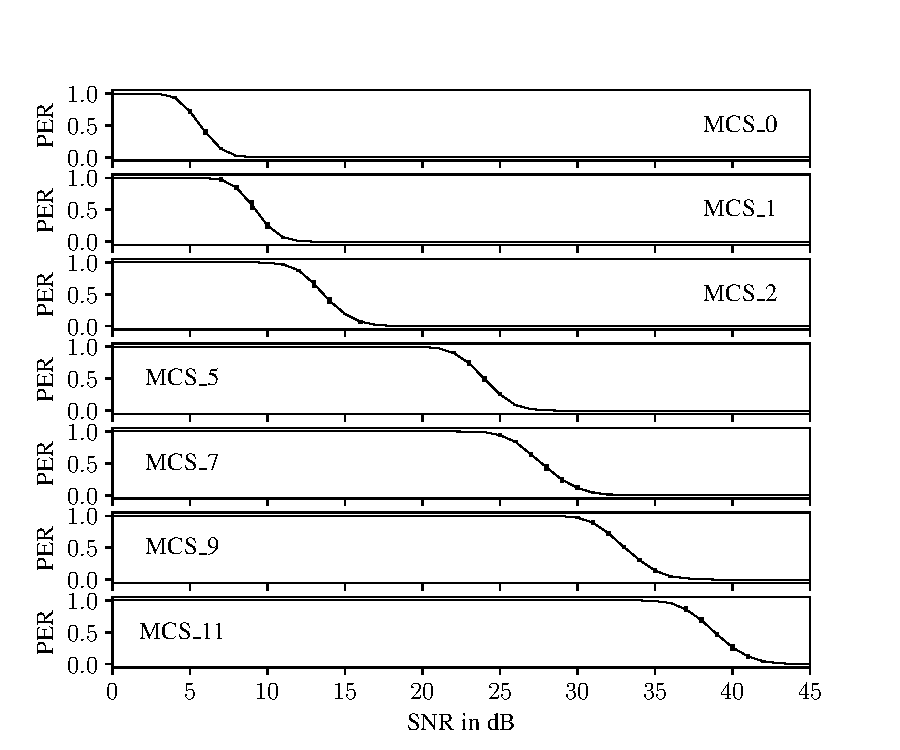
\includegraphics[width=0.95\textwidth]{figures/MCS_PER_to_SNR.pdf}
	\caption{Achieved Goodput and theoretical Datarate of two WiFi 6 stations in Ad-Hoc Mode with a \ac{GI} of \SI{3200}{\nano\second} and a bandwidth of \SI{40}{\mega\hertz} in regards to the number of the chosen \ac{MCS} and \ac{CR} and whether \ac{DCM} is enabled}%
	\label{fig:PER_SNR_MCS}%
\end{figure}

\subsubsection*{\acf{FEC}}
Another parameter that influences the \ac{PER} is the choice of the forward error correction (FEC) procedure. In order to
analyse the influence of the FEC procedure on the \ac{PER}, I simulated the \ac{PER} in regards to the \ac{SNR} for HE-MCS
\numrange{0}{9} and whether \ac{LDPC} or \ac{BCC} is enabled. For higher HE-MCS values \ac{BCC} can be used as \ac{LDPC} is compulsory, so no comparison of the \ac{FEC} procedures is possible.

The results are displayed in \autoref{fig:PER_SNR_LDPC}. The \ac{PER} decreases with higher \ac{SNR} for both \ac{FEC} procedures for all HE-MCS values as
expected. Using \ac{LDPC} instead of \ac{BCC} decreases the \ac{PER} for all HE-MCS values at lower \ac{SNR} values.
\begin{figure}[H]%
	\centering
	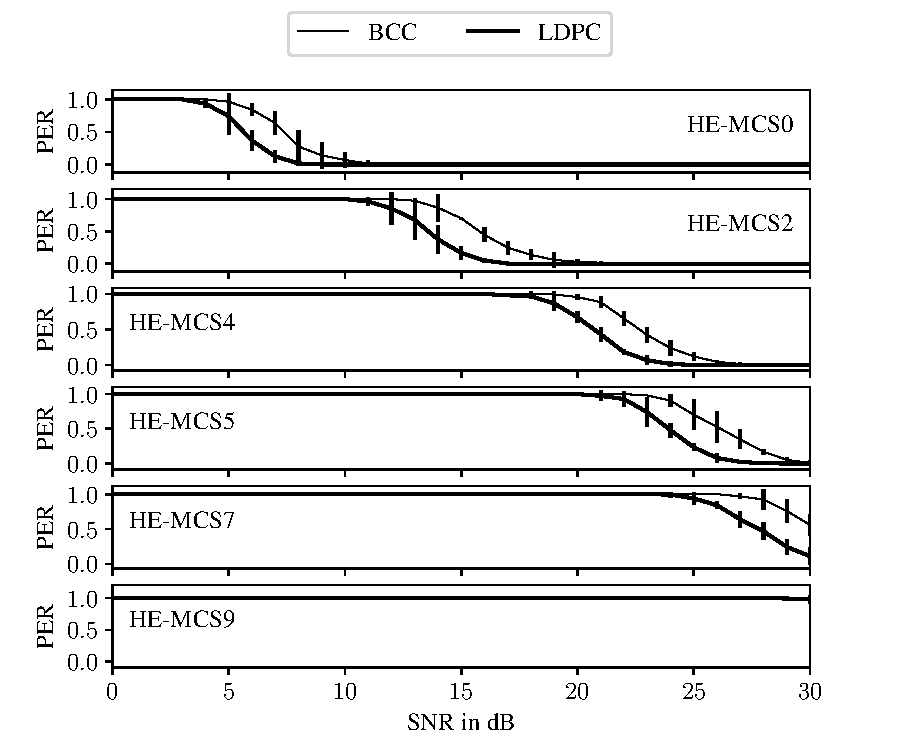
\includegraphics[width=0.95\textwidth]{figures/LDPC_PER_to_SNR.pdf}
	\caption{Simulated \ac{PER} in regards to \ac{SNR} for chosen HE-\ac{MCS} values and whether \ac{LDPC} or \ac{BCC} is enabled for IEEE 802.11ax physical layer parameters of a \ac{GI} of \SI{3200}{\nano\second}, a bandwidth of \SI{20}{\mega\hertz} and 2 spatial streams}%
	\label{fig:PER_SNR_LDPC}%
\end{figure}

\subsubsection*{\acf{GI}}
\begin{figure}%
	\centering
	
\includegraphics[width=0.95\textwidth]{figures/GI_PER_to_SNR.pdf}
	\caption{Achieved Goodput and theoretical Datarate of two WiFi 6 stations in Ad-Hoc Mode with a \ac{GI} of \SI{3200}{\nano\second} and a bandwidth of \SI{40}{\mega\hertz} in regards to the number of the chosen \ac{MCS} and \ac{CR} and whether \ac{DCM} is enabled}%
	\label{fig:PER_SNR_GI}%
\end{figure}
\cite{patil} effect

cite others seane old??



\subsubsection*{\acf{DCM}}
Next, I simulated the \ac{PER} in regards to the \ac{SNR}  and whether \ac{DCM} is enabled for the specfied HE-\ac{MCS} values. Dabei habe ich für die SImulation die möglichen
HE-MCS \num{0},\num{1},\num{3} and \num{4} aus dem IEEE 802.11ax Standard verwendet.

The results indicate, that using \ac{DCM} can achieve the same \ac{PER} at lower \ac{SNR} values compared to not using \ac{DCM}. \ac{DCM} also influenced the
\ac{PER} to decrease at lower a \ac{SNR} for all specified HE-MCS values. The results are visualized in \autoref{fig:PER_SNR_DCM}.
\begin{figure}[H]%
	\centering
	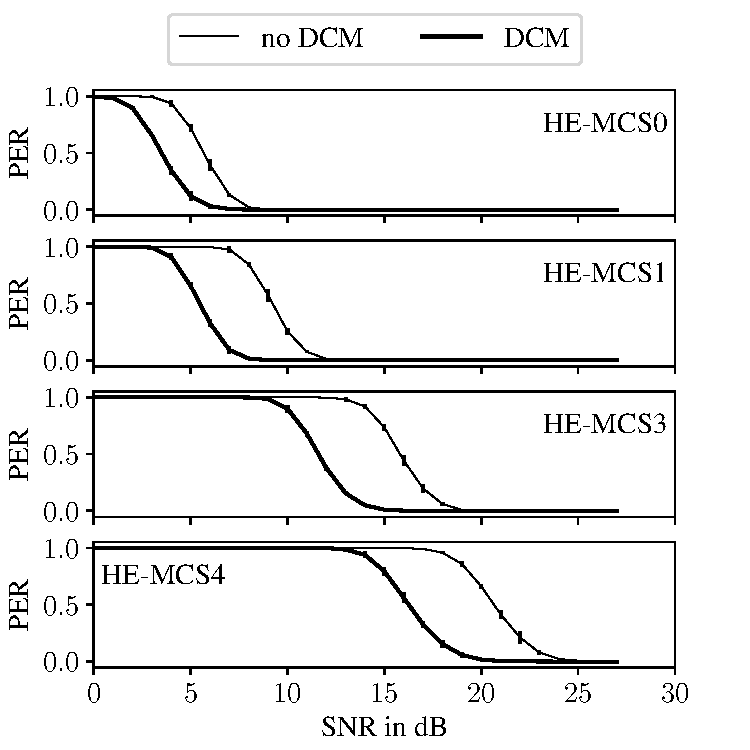
\includegraphics[width=0.95\textwidth]{figures/DCM_PER_to_SNR.pdf}
	\caption{Simulated \ac{PER} in regards to \ac{SNR} for chosen HE-\ac{MCS} values and whether \ac{DCM} is enabled for IEEE 802.11ax physical layer parameters of a \ac{GI} of \SI{3200}{\nano\second}, a \ac{BW} of \SI{20}{\mega\hertz} and 2 spatial streams}%
	\label{fig:PER_SNR_DCM}%
\end{figure}


\Textcite{ryu_ber_2010} and \textcite{park_ber_2006} conducted a similar simulation, where they analyse the bit error rate in
regards to the normalized \ac{SNR} and whether \ac{DCM} was enabled for rayleigh fading channels. Both authers wraped two
Quadrature \ac{PSK} modulated symbols into one 16-\ac{QAM} symbol. As Quadrature \ac{PSK} modulates \SI{2}{\bit} per symbol, the infomation
of two Quadrature \ac{PSK} modulated symbols can be
transmitted in one 16-\ac{QAM} symbol, which encodes \SI{4}{\bit}. The authors transmit the 16-\ac{QAM} symbols and a redundant copy
of the 16-\ac{QAM} symbols via orthogonal subcarriers. At the receiver the authors combine the copies and retrieve the transmitted
information using the Maximum likelyhood criterion. The results of the author show that a better bite error rate can be achieved while applying
\ac{DCM} than sending the information via two Quadrature \ac{PSK} or 16-\ac{QAM} modulated symbols without \ac{DCM}.


\todo[color=yellow]{name PER 0.5 Some paper use  0.1 is very good Sommerf0.1 PER and mention the SNR improvement 4 db improvement}
\subsubsection*{\acf{ER}}
For a HE-MCS \num{0} and \num{1} the \ac{ER} range mode can be applied additional to \ac{DCM}, when one spatial stream is used \cite{noauthor_ieee_2021}.
In order to analyse the impact of the \ac{ER} mode, I set the physical layer parameters to a \ac{GI} of
\SI{3200}{\nano\second}, a \ac{BW} of \SI{20}{\mega\hertz} and one spatial streams. For He-MCS \num{0}, \num{1} and \num{3} I run simulations, where I enabled the
\ac{ER} mode and compared the \ac{PER} to the \ac{PER} of the same HE-MCS values without \ac{ER} mode.
The results in \autoref{fig:PER_SNR_ER} indicate , that the \ac{PER} is influenced by the \ac{ER} mode. The \ac{PER} decreases with at lower \ac{SNR} for all HE-MCS values
when \ac{ER} is enabled.
\begin{figure}%
	\centering
	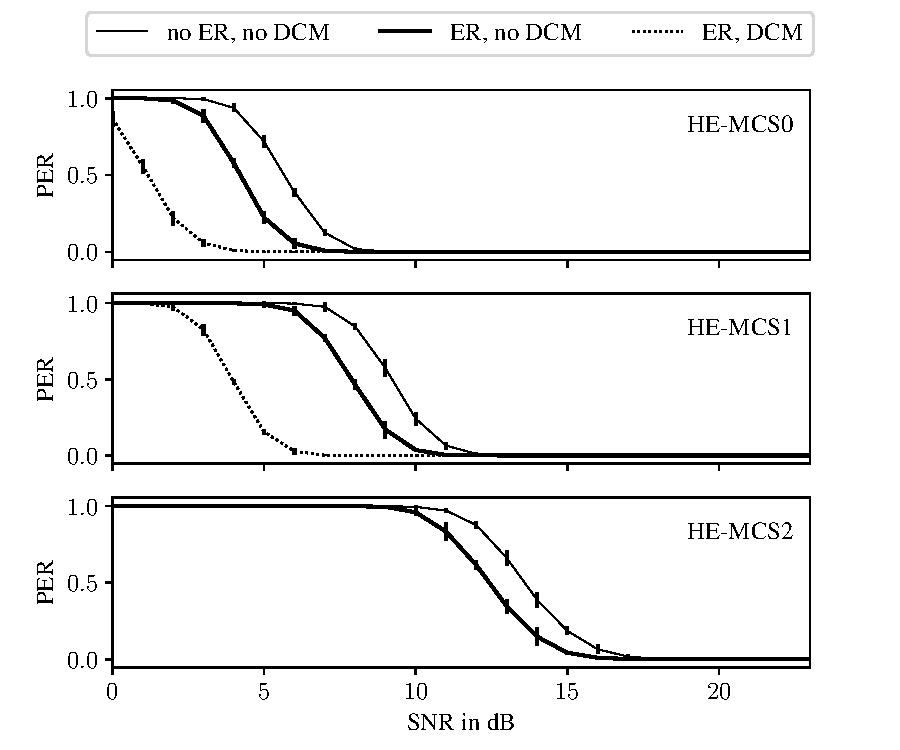
\includegraphics[width=0.95\textwidth]{figures/ER_PER_to_SNR.pdf}
	\caption{Simulated \ac{PER} in regards to \ac{SNR} for chosen HE-\ac{MCS} values and whether Extended Range or \ac{DCM}
	is enabled for IEEE 802.11ax physical layer parameters of a \ac{GI} of \SI{3200}{\nano\second}, a \ac{BW} of \SI{20}{\mega\hertz} and 2 spatial streams}
	\label{fig:PER_SNR_ER}%
\end{figure}
Additionally, I simulated the impact of applying the \ac{ER} mode and \ac{DCM} for the allow HE-MCS values \num{0} and \num{1}.
Applying \ac{DCM} additionally makes the transmission more robust and decreases the \ac{PER} at even lower \ac{SNR} as
it is displayed in \autoref{fig:PER_SNR_ER_DCM}.

\textcite{jacob_system-level_2020} conducted a simulation, where they analysed the effect of \ac{DCM} and \ac{ER} on the \ac{PER} for
IEEE 802.11bd in vehicular environments to the transmission range. The authors found out, that the using \ac{DCM} and \ac{ER} can
increase the transmission range for \ac{LoS} by \SI{65}{\percent} for a \ac{PER} greater than \num{0.1}. After additional analysis with higher
vehicle densities, the authors remark, that using \ac{DCM} and the \ac{ER} mode cause channel congestion in CSMA/CA based
networks with low bandwidths. The authors conclude, that the \ac{ER} mode and \ac{DCM} should be used for long range transmissions, where
the physical layer parameters can extend the transmission range significantly.

A similar simulation was conducted by \textcite{triwinarko_phy_2021}. The researchers state, that using \ac{DCM} and the
\ac{ER} mode results in better \ac{PER} performance at lower \ac{SNR} values in \ac{LoS} and non \ac{LoS} scenarios.

\subsubsection*{\acf{STBC}}

\begin{figure}%
	\centering
	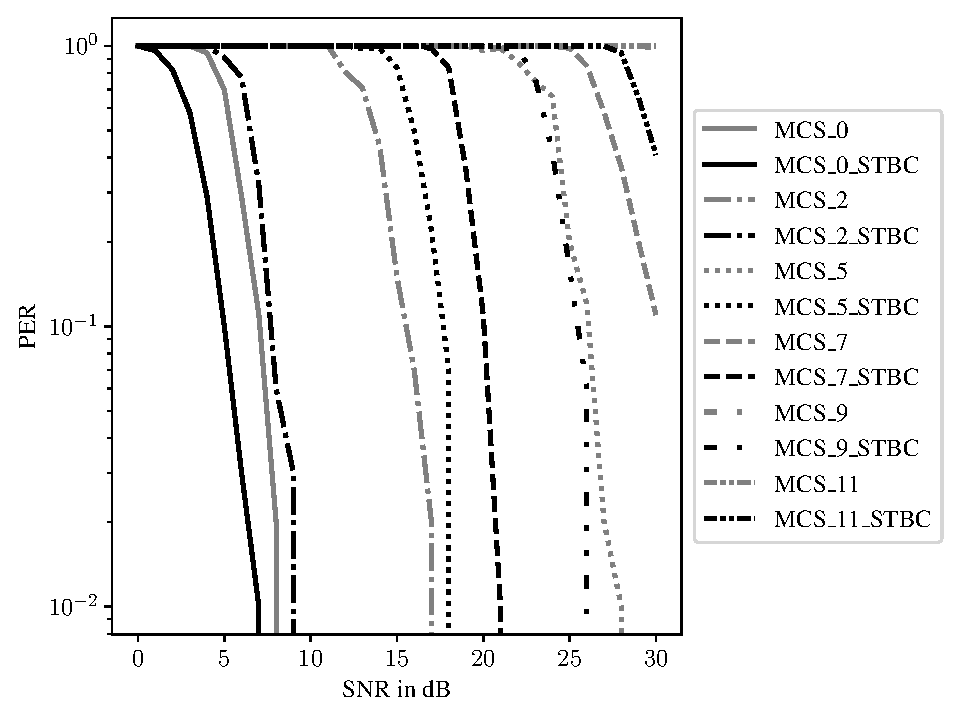
\includegraphics[width=0.95\textwidth]{figures/STBC_PER_to_SNR.pdf}
	\caption{Simulated \ac{PER} in regards to \ac{SNR} for chosen HE-\ac{MCS} values and whether \ac{STBC} is enabled for IEEE 802.11ax physical layer parameters of a \ac{GI} of \SI{3200}{\nano\second}, a \ac{BW} of \SI{20}{\mega\hertz} and 2 spatial streams}%
	\label{fig:PER_SNR_STBC}%
\end{figure}